\documentclass[11pt]{article}

\usepackage{tikz}
\usetikzlibrary{arrows}
\usepackage[margin=1in]{geometry}
\usepackage{listings}
\usepackage{color}
\usepackage{program}



\title{Cyberinfrastructure Foundations: Final}
\author{Matthew Le}

\begin{document}
\maketitle

1. (5 points) Discuss how cyberinfrastructure will change science and engineering research in your domain with justifications.

{\bf My research revolves around designing programming languages that allow programmers to easily develop parallel applications.  As parallel architectures evolve, the compilers and runtime systems for these languages must evolve with them.  }\\


2. (5 points)Middleware enables remote method invocation for distributed objects, so that a thread can use remote objects like local ones. Java RMI is one of them. Discuss in detail how Java RMI makes this possible. Use a diagram and discuss each component briefly.

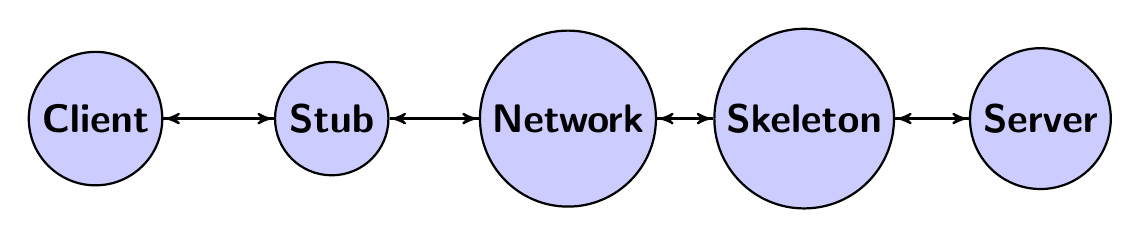
\begin{tikzpicture}[->,>=stealth',shorten >=1pt,auto,node distance=3cm,
  thick,main node/.style={circle,fill=blue!20,draw,font=\sffamily\Large\bfseries}]
  
  \node[main node] (Client){Client};
  \node[main node] (Stub)[right of=Client]{Stub};
  \node[main node] (Network)[right of=Stub]{Network};
  \node[main node] (Skeleton)[right of=Network]{Skeleton};
  \node[main node] (Server)[right of =Skeleton]{Server};
  
  \path[every node/.style={font=\sffamily\small}]
  	(Client) edge node [left]{} (Stub)
	(Stub) edge node [right]{}(Client)
	(Stub) edge node [right]{}(Network)
	(Network) edge node [right]{}(Stub)
	(Network) edge node [right]{}(Skeleton)
	(Skeleton) edge node [left]{}(Network)
	(Skeleton) edge node [right]{}(Server)
	(Server) edge node [right]{}(Skeleton)
	;
  
\end{tikzpicture}


7. (5 points) Breadth-first search conducts exhaustive search that visits all of the nodes in a graph. This is why breadth-first search is a popular algorithm for problem solving. Give a sketch of the breadth-first search algorithm. Your sketch must be specific like pseudo- code.

\begin{figure}[h]

\begin{program}
\PROC bfs(G, s) \BODY

	Q = EmptyQueue;
	Q.deque(s);
	\WHILE(!Q.isEmpty()) \DO
		n = Q.deque()
		n.seen = true;
		\FOR v\; |in| \; neighbors(n)\; \DO
			Q.enque(v);
		\END
	\END
	
\END
\end{program}

\end{figure}


\end{document}






